\section{Methodology}
\label{sec:methodology}

The pruning problem can be seen as finding an optimal mask under a sparsity constraint.
However, without retraining, the problem becomes intractable.
To address this, we decompose Transformer pruning into three sub-problems, each of which can be efficiently solved; the first two stages of our pipeline address the problems of finding an optimal \textit{binary} mask, and the last stage further optimizes it into a \textit{real-valued} mask.

Note that the number of the mask variables is much less than the number of the parameters in a Transformer (e.g., 37K vs. 110M in case of BERT$_\textsc{base}$).
This allows the framework to use only a small number of examples without overfitting to the sample dataset, and thus to be extremely faster than the retraining-based pruning methods which typically use the entire dataset.
As the framework keeps the model ``as is'' and only decides the mask variables, we henceforth regard the model parameters as constants and consider the mask variables as the only parameters for our pruning problem.

\textbf{Problem Formulation.}
We formulate Transformer pruning as a constrained optimization problem on the mask $\text{m}$:
\begin{align}
% \small
    \argmin_{\text{m}} \loss(\text{m}) \label{eq:original_objective} \quad \text{s.t.} \quad \text{Cost}(\text{m}) \leq C
\end{align}
where $\loss$ denotes the loss function, $\text{Cost}$ is the FLOPs/latency of the architecture pruned by the mask, and $C$ is the given FLOPs/latency constraint.
Unfortunately, such a problem is generally intractable as $\text{Cost}$ is usually a function of $l_0$-norm of the mask $\text{m}$, which is non-differentiable.
Thus, in what follows, we introduce several assumptions and approximations to simplify the~problem.

We start by approximating the loss function using the second-order Taylor expansion around the initial mask  $\mathbb{1}$:
\vspace{-2mm}
\begin{align}
% \small
    \loss(\text{m}) & \approx \loss(\mathbb{1}) - \text{g}^\intercal (\mathbb{1} - \text{m}) + \frac{1}{2}(\mathbb{1} - \text{m})^\intercal \text{H} (\mathbb{1} - \text{m}) \\
    &\approx \loss(\mathbb{1}) + \frac{1}{2}(\mathbb{1} - \text{m})^\intercal \text{H} (\mathbb{1} - \text{m}) , \label{eq:lm_nograd}
\end{align}
where $\text{g} = \mathbb{E}[\frac{\partial}{\partial \text{m}} \loss(\mathbb{1})]$ and $\text{H} = \mathbb{E}[\frac{\partial^2}{\partial \text{m}^2} \loss(\mathbb{1})]$.
\eref{eq:lm_nograd} is deduced from an assumption that the model has converged to a local minima, where the gradient term is close to 0~\cite{lecun1990optimal}.
As $\loss(\mathbb{1})$ is a constant, we can rewrite the optimization objective as follows:
\begin{align}
% \small
    \argmin_{\text{m}} \loss(\text{m}) 
    \approx \argmin_{\text{m}} (\mathbb{1} - \text{m})^\intercal \text{H} (\mathbb{1} - \text{m}). \label{eq:argmin_hessian}
\end{align}
\eref{eq:argmin_hessian} shows that the optimal mask is determined by the Hessian of the loss with respect to the mask variables.
Since forming the exact Hessian matrix explicitly is infeasible, we approximate the Hessian $\text{H}$ with the (empirical) Fisher information matrix $\mathcal{I}$ of the mask~variables:
\begin{align}
\small
    \mathcal{I} := \frac{1}{|\mathcal{D}|} \sum_{(x, y) \in \mathcal{D}} \big(\frac{\partial}{\partial \text{m}}\loss(x, y; \mathbb{1})\big) \big(\frac{\partial}{\partial \text{m}}\loss(x, y; \mathbb{1})\big)^\intercal, \label{eq:fim}
\end{align}
where $\mathcal{D}$ is the sample dataset and $(x, y)$ is a tuple of an input example and its label.

\subsection{Fisher-based Mask Search}
\label{subsec:search}

\textbf{Diagonal Approximation of the Fisher Information Matrix.}
It is intractable to solve the optimization objective in~\eref{eq:argmin_hessian} using the full Fisher information matrix $\mathcal{I}$.
Thus, we first make a simple assumption that $\mathcal{I}$ is \textit{diagonal}.
This further simplifies \eref{eq:argmin_hessian} as follows:
\begin{gather}
% \small
    \argmin_{\text{m}} \loss(\text{m}) \approx \argmin_{\text{m}} \sum_i (1 - m_i)^2 \mathcal{I}_{ii}, \label{eq:argmin_importance}
\end{gather}
Since we restrict the possible mask values to either 0 or 1, the following can be derived from \eref{eq:argmin_importance}:
\begin{gather}
% \small
    \argmin_{\text{m}} \loss(\text{m}) \approx \argmin_{\text{m}} \sum_{i \in Z(\text{m})} \mathcal{I}_{ii} \label{eq:sum_importance} \quad
    \text{where} \quad Z(\text{m}) := \{i \ | \ m_i = 0 \}.
\end{gather}
We can interpret each diagonal element of $\mathcal{I}$ as the \textit{importance score} of the head/filter associated with the mask variable,
and \eref{eq:sum_importance} as a process of minimizing the total importance scores of the pruned heads and filters.
Such an importance score has also been introduced in~\cite{molchanov2019importance, theis2018faster} to guide pruning.

\setlength{\textfloatsep}{6pt}
\begin{algorithm}[tb]
   \caption{Mask Search with a FLOPs Constraint}
   \label{alg:search_flops}
   
% \footnotesize
    {\bfseries Input:} FLOPs constraint $C$, diagonal Fisher information matrix $\mathcal{I}$
   
\begin{algorithmic}[1]
    \STATE \textbf{for} {$n=0$ {\bfseries to} $LH$} \textbf{do} \label{alg:search_flops:for} 
    \hspace*{\fill}{$\triangleright$ \# remaining heads}
        \STATE \quad  $k_1 = LH - n$ \hspace*{\fill}{$\triangleright$ \# heads to prune}
        \STATE \quad $\text{HI} = $ indicies of $k_1$ least important heads
        \STATE \quad $f = \lfloor (C - n \text{F}_{\text{head}}) / \text{F}_\text{filter} \rfloor $ \label{alg:search_flops:num_filters}
        \hspace*{\fill}{$\triangleright$ \# remaining filters}
        \STATE \quad $k_2 = LN - f$
        \hspace*{\fill}{$\triangleright$ \# filters to prune}
        \STATE \quad $\text{FI} = $ indicies of $k_2$ least important filters
        \STATE \quad $S[n] = \sum_{i \in \text{HI} \cup \text{FI}} \mathcal{I}_{ii}$
        \STATE \quad $R[n] = (\text{HI}, \text{FI})$
        % \STATE \quad $R[n] = (\text{HI}, \text{FI})$
    \STATE \textbf{end for}
    \STATE $n^\ast = \argmin_n S[n]$
    \hspace*{\fill}{$\triangleright$ optimal \# remaining heads} \label{alg:search_flops:argmin_s}
    \STATE $\text{HI}^\ast, \text{FI}^\ast = R[n^\ast]$ \label{alg:search_flops:r_n}
    \hspace*{\fill}{$\triangleright$ indicies of heads/filters to prune}
    \STATE Initialize $\text{m}^{\textsc{MHA}}$ and $\text{m}^{\textsc{FFN}}$ as $\mathbb{1}$
    \STATE $\text{m}^{\textsc{MHA}}[\text{HI}^\ast] = 0$ \hspace*{\fill}{$\triangleright$ prune the selected heads}
    \STATE $\text{m}^{\textsc{FFN}}[\text{FI}^\ast] = 0$ \hspace*{\fill}{$\triangleright$ prune the selected filters}
\end{algorithmic}

     {\bfseries Output:} $\text{m}^\ast = (\text{m}^{\textrm{MHA}}$, $\text{m}^{\textrm{FFN}})$
\end{algorithm}

\textbf{Solving FLOPs-constrained Problem.}
We need to solve~\eref{eq:sum_importance} given a cost constraint.
For a given target FLOPs cost, denoted by C, we can formulate the binary mask search problem as follows:
\begin{gather}
% \small
    \argmin_{\text{m}} \sum_{i \in Z(\text{m})} \mathcal{I}_{ii} \quad
    \text{s.t.} \quad \text{F}_{\text{head}} || \text{m}^{\textsc{mha}} ||_0 + \text{F}_{\text{filter}} || \text{m}^{\textsc{ffn}} ||_0 \leq C \label{eq:flops_objective},
\end{gather}
where $\text{F}_\text{head} \in \mathbb{R}$ and $\text{F}_\text{filter} \in \mathbb{R}$  are the FLOPs for computing a head and a filter, respectively.
Note that the number of FLOPs of a head/filter is constant across all layers.
While such an optimization problem can be generally solved by a knapsack algorithm~\cite{aflalo2020knapsack, shen2021halp}, the following observations allow a faster polynomial-time solution:
(1) having more heads and filters unpruned always optimizes \eref{eq:flops_objective} since the diagonal elements of $\mathcal{I}$ are non-negative; and
(2) if a certain number of heads needs to be pruned, they should be the ones with the lowest importance scores because each head accounts for the same amount of FLOPs.
The same statement also holds for pruning filters.
The two observations lead to our mask search algorithm described in Algorithm~\ref{alg:search_flops}.

Algorithm~\ref{alg:search_flops} partitions the solution space by the total number of remaining heads in the pruned architecture ($n$ in line~\ref{alg:search_flops:for}).
For each $n$, the number of remaining filters should be the largest possible number that satisfies the cost constraint by observation (1), which can be described as $f$ in line~\ref{alg:search_flops:num_filters}.
Then by observation (2), the heads/filters with the lowest important scores are selected to be pruned. 
Therefore, $S[n]$ is a solution of~\eref{eq:flops_objective} under additional constraint of fixing the number of remaining heads to be $n$.
When the loop terminates, 
the output is the mask that minimizes $S[n]$ across all possible $n$ (line~\ref{alg:search_flops:argmin_s} and \ref{alg:search_flops:r_n}).
In~\sref{appendix:optimality_proof}, we prove that
the output mask $\text{m}^\ast$ of Algorithm~\ref{alg:search_flops} is optimal.
That is, any other mask $\text{m}$ satisfying the given FLOPs constraint will result in a higher loss:
\begin{equation}
\label{eqn:from_theorem:optimal_mask}
   \sum_{i \in Z(\text{m}^\ast)} \mathcal{I}_{ii} \leq \sum_{i \in Z(\text{m})} \mathcal{I}_{ii}.
\end{equation}

% \vspace{-2mm}
\textbf{Solving Latency-constrained Problem.}
If the cost constraint is given in terms of latency on target hardware, 
we have a new optimization problem with a different cost constraint than \eref{eq:flops_objective}:
\begin{gather}
% \small
    \argmin_{\text{m}} \sum_{i \in Z(\text{m})} \mathcal{I} \label{eq:latency_objective} \quad
    \text{s.t.} \quad \sum_{l=1}^L \text{LAT}(\text{m}^{\textsc{mha}}_l) + \sum_{l=1}^L \text{LAT}(\text{m}^{\textsc{ffn}}_l) \leq C,
\end{gather}
where the function $\text{LAT}$ indicates the latency of a MHA/FFN layer after pruning.
We assume that a latency lookup table on the target hardware is provided so that evaluating $\text{LAT}$ takes negligible time.

Unfortunately, the latency constraint makes the problem more challenging 
as directly applying Algorithm~\ref{alg:search_flops} is no longer possible.
This is because $\text{LAT}$ is \textit{not} linear to the number of remaining heads or filters after pruning~\cite{radu2019performance}, as shown in \fref{fig:lat} (Left).
We can interpret this as follows:
(1) with a sufficient number of heads/filters in a layer, the hardware resources such as parallel cores can be fully utilized, resulting in latency roughly proportional to the number of heads/filters; and
(2) otherwise, the hardware is underutilized and a constant overhead dominates the latency~\cite{kwon2020nimble, ma2020rammer}.
Thus, pruning more heads/filters below a certain threshold does not translate into actual speedup.


%%%%%%%%%%%%%%%%%%%%%%%%%%%%%%%%%%%%%%%%%%%%%%%%%%%%%%%%%%%%%%%%%%%%%%%%%%%%%%
\begin{table}[!t]
	\begin{minipage}{0.62\linewidth}
    \vspace{8mm}
		\begin{center}
    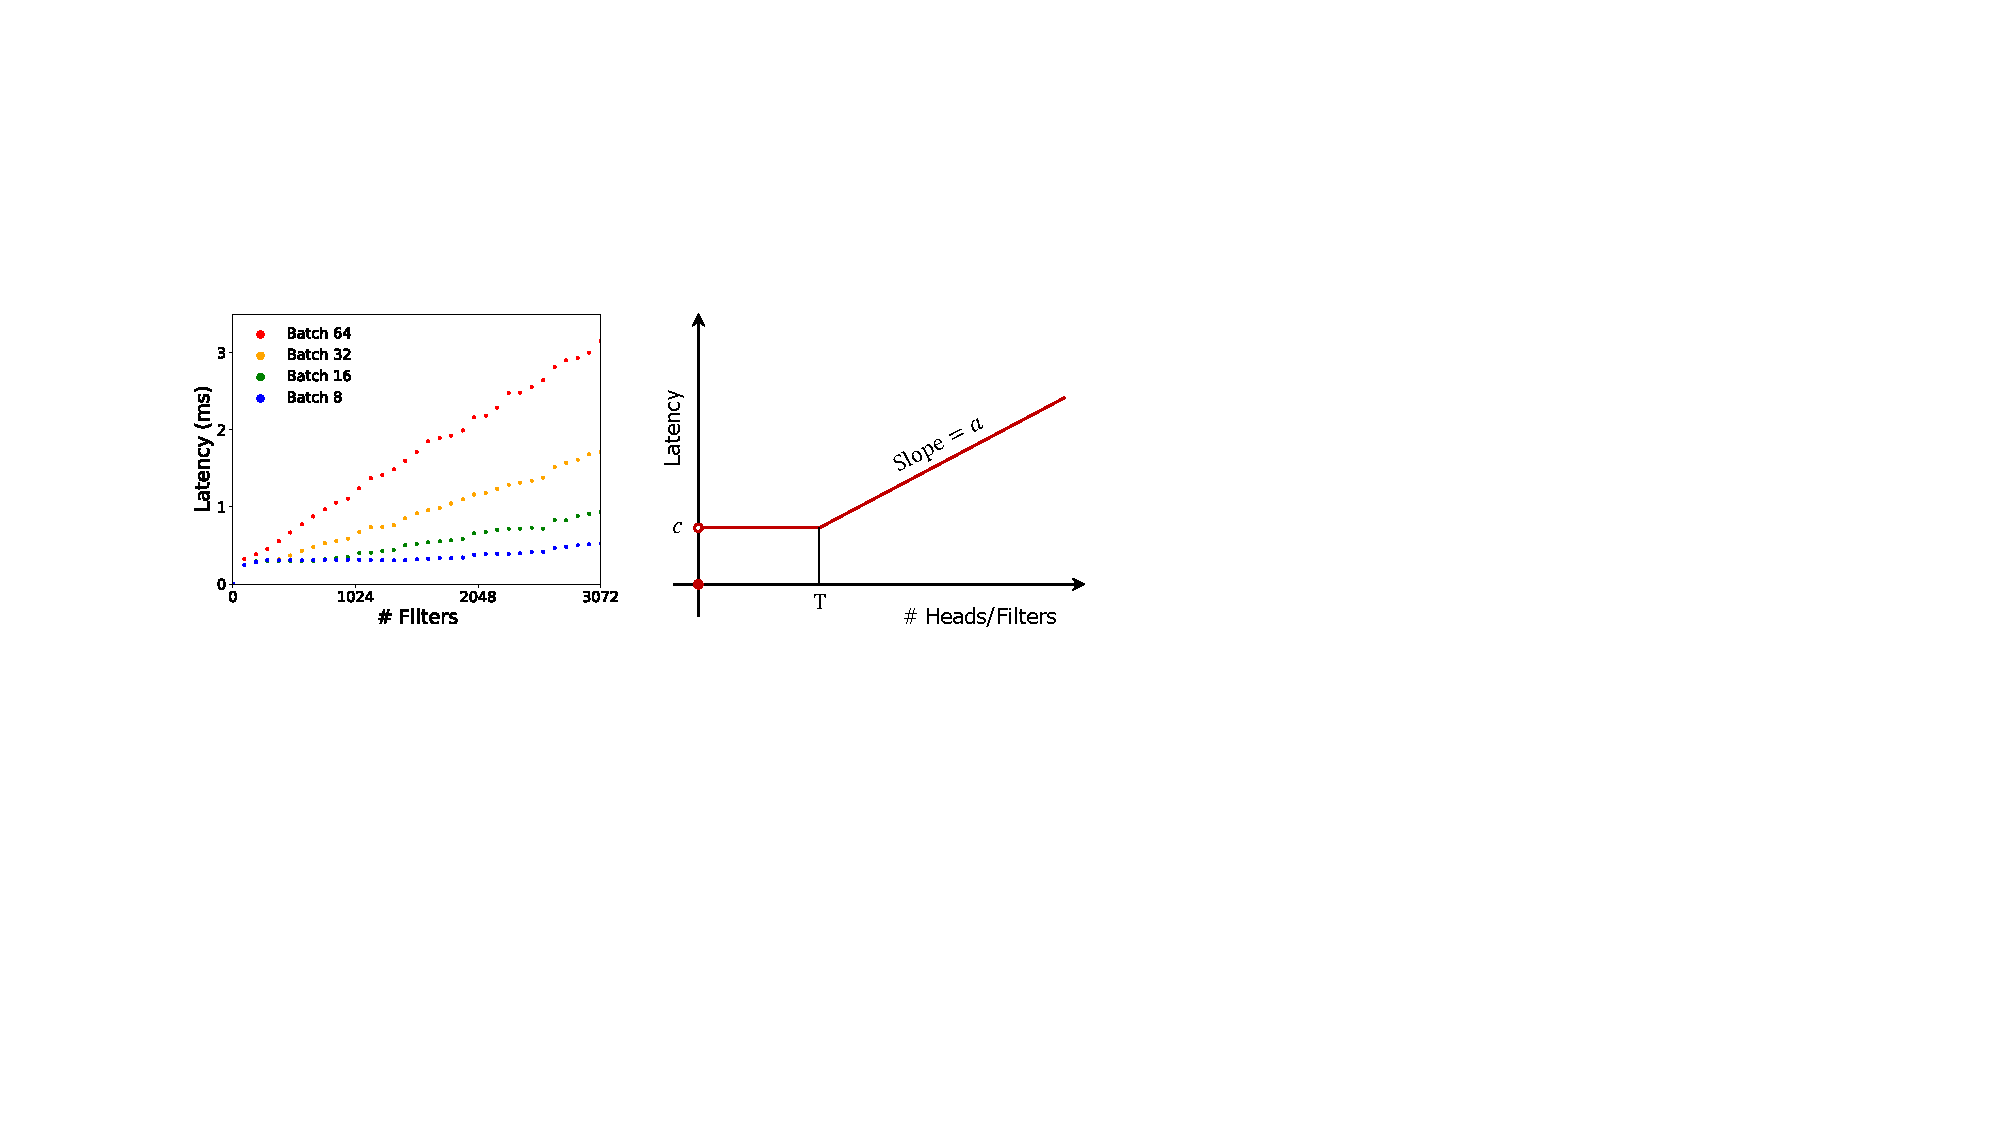
\includegraphics[width=1\columnwidth]{figures/latency.pdf}
  \end{center}
    \captionof{figure}{
    (Left) Real latency of a single FFN layer with different numbers of remaining filters. (Right) Schematic plot for the approximated latency as a piece-wise linear function.}
    \label{fig:lat}
	\end{minipage}
	\hfill
	\begin{minipage}{0.33\linewidth}
  \begin{center}
    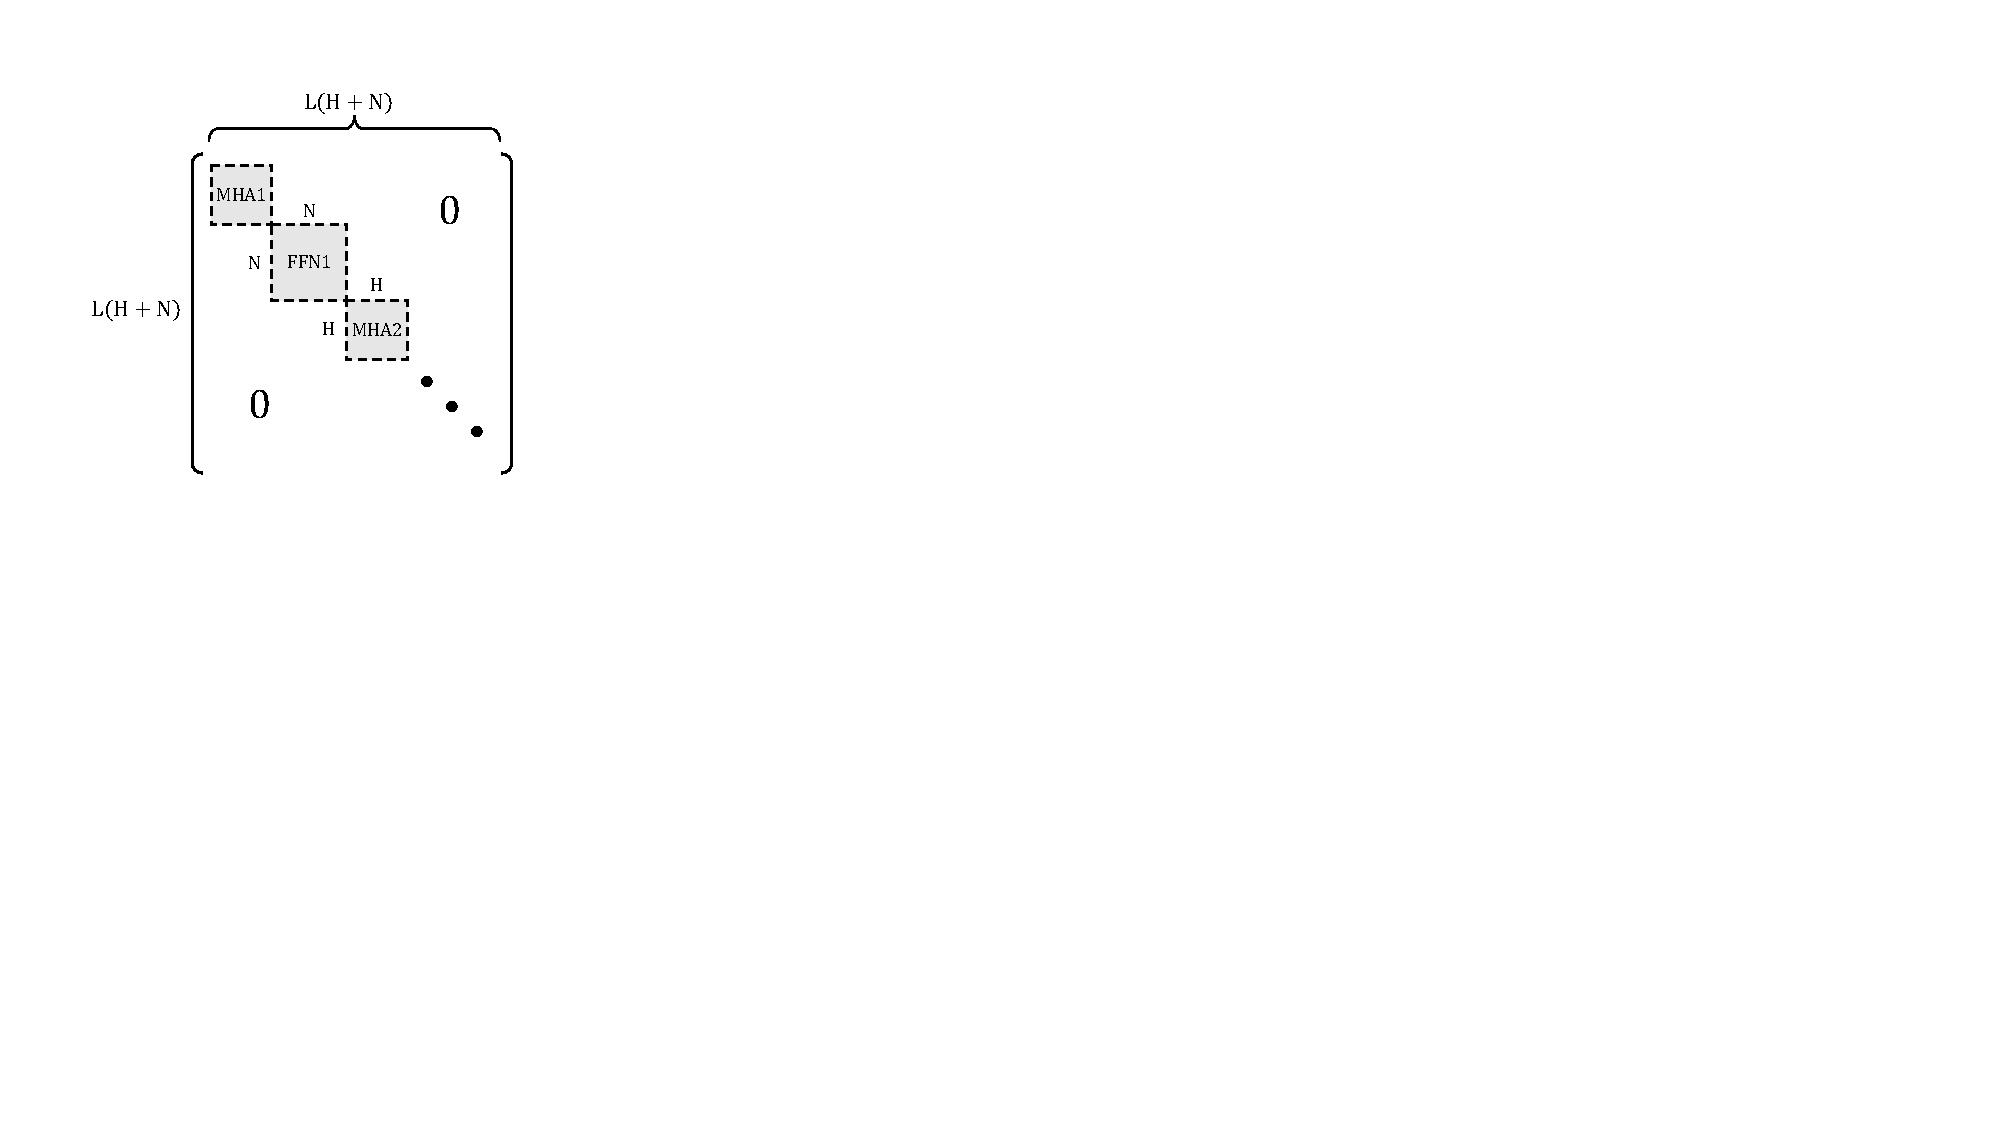
\includegraphics[width=1\columnwidth]{figures/fisher.pdf}
  \end{center}
  \captionof{figure}{
    Illustration of the block diagonal Fisher matrix.
    }
\label{fig:block-diagonal}
	\end{minipage}
	\vspace{-3mm}
\end{table}
%%%%%%%%%%%%%%%%%%%%%%%%%%%%%%%%%%%%%%%%%%%%%%%%%%%%%%%%%%%%%%%%%%%%%%%%%%%%%%


Based on the above analysis, we approximate $\text{LAT}$ as a piece-wise linear function as in \fref{fig:lat} (Right)
such that $\text{LAT}(\text{m}_l)$ is 0 if $||\text{m}_l||_0 = 0$,
$c$ if $0 < ||\text{m}_l||_0 \leq T$, and 
$a(||\text{m}_l||_0 - T) + c \ $ if $||\text{m}_l||_0 > T$,
where $c \in \mathbb{R}$ is the constant overhead, $T \in \mathbb{N}$ is the threshold number of heads/filters that the latency starts to become linear, and $a \in \mathbb{R}$ is the slope of the linear part.
This can be easily obtained by fitting the actual latency data in the lookup table with the minimum mean squared error.

The piece-wise linear approximation of $\text{LAT}$ allows us to extend Algorithm~\ref{alg:search_flops} to the setting with latency constraints.
The core idea is to separately consider the constant part and the linear part of $\text{LAT}$; after handling the constant part, we can apply the Algorithm~\ref{alg:search_flops} to the linear part.
The detailed modification to Algorithm~\ref{alg:search_flops} is described in~\sref{appendix:latency_algorithm}.

\vspace{-2mm}
\subsection{Fisher-based Mask Rearrangement}
\label{subsec:rearrange}
\vspace{-1mm}

\textbf{Block Diagonal Approximation of the Fisher Information Matrix.}
Although it simplifies the problem, the diagonal assumption in \sref{subsec:search} alone might not find the best solution, as it does not take into account the interactions between different mask variables.
For example, if there are two attention heads playing a similar role in a layer, pruning only one of them might not affect the model accuracy.
However, when both of them are pruned, the model accuracy can be significantly degraded.
Such interactions are captured by the non-diagonal elements of the Fisher information matrix, which were ignored in the previous stage.
Thus, we can better consider the interactions in our pruning problem by using a \textit{block diagonal} approximation to the Fisher matrix, where a block corresponds to a MHA layer or a FFN layer as illustrated in~\fref{fig:block-diagonal}.

However, the block diagonal approximation results in an intractable optimization problem over the binary mask.
To alleviate this, we use the results from the previous stage to \textit{warm start} the optimization problem.
First, we constrain the number of heads/filters to prune for each layer to be the same as the binary mask we obtained in the first stage.
In other words, given the mask $\text{m}^\ast$ obtained in \sref{subsec:search}, we constrain 
$|| \text{m}_l ||_0$ to be equal to  $||\text{m}^{\ast}_l ||_0 $ for each layer $l$.
Second, we use the mask $\text{m}^\ast$ as the starting point of the greedy search to solve the new optimization problem. 

Given the two assumptions that (i) there is no interaction between the mask variables in different layers (i.e., the block diagonal approximation), and (ii) the number of heads/filters to prune are pre-determined for each layer (i.e., warm-start), \eref{eq:argmin_hessian} breaks down to a set of \textit{layer-wise} optimization problems, as follows based on the derivation in~\sref{appendix:derivation_block_diagonal}:
\begin{gather}
% \small
    {\hat{\text{m}}}_l = \argmin_{\text{m}_l} (\mathbb{1} - \text{m}_l)^\intercal \mathcal{I}_l (\mathbb{1} - \text{m}_l), \label{eq:layerwise_opt}
\end{gather}
where $\mathcal{I}_l$ is the $l$-th diagonal block of $\mathcal{I}$.
We approximately solve this problem with a greedy algorithm.
After initializing the mask $\text{m}_l$ as $\text{m}^{\ast}_l$ (i.e., warm-start),
we pick for every round a pruned head (or filter) with the highest Fisher information and exchange it with an unpruned head (or filter) in the current mask if that can further optimize \eref{eq:layerwise_opt}.
After every pruned head/filter goes through one round, we obtain an approximate solution to \eref{eq:layerwise_opt}.

Because this process does not change the number of heads/filters in each layer, the obtained mask $\hat{\text{m}}_l$ results in the same FLOPs/latency as that of the mask $\text{m}^{\ast}_l$ searched in~\sref{subsec:search}.
In effect, this process \textit{rearranges} the binary mask variables of each layer to find a better arrangement of pruning locations and capture the intra-layer interactions. 

\subsection{Mask Tuning}
\label{subsec:tuning}
\vspace{-1mm}

In the previous two stages, the possible mask values are restricted to either 0 or 1 in order to simplify the search process.
In this stage, we further relax this restriction.
The \textit{nonzero} variables in the mask $\hat{\text{m}}$ from \sref{subsec:rearrange} are tuned to any real values such that the pruned model recovers its accuracy.

\textbf{Layer-wise Reconstruction via Linear Least Squares.}
We tune the mask variables toward minimizing the \textit{layer-wise reconstruction error}, similarly to~\cite{he2017channel}.
From the first to the last layer, we reconstruct the output activation of the original model with the remaining heads/filters in the pruned model.
This can be formally written as follows:
\vspace{-1mm}
\begin{gather}
% \small
    \argmin_{\text{m}_l} || \text{x}  + \mathrm{layer}(\text{x}; \text{m}_l) - \big(\text{x}' + \mathrm{layer}(\text{x}'; \mathbb{1})\big) ||_2^2, \label{eq:reconstruction}
\end{gather}
where $\mathrm{layer}$ is either MHA or FFN, and $\text{x}$ and $\text{x}'$ are the inputs to the layer of the pruned model and the original model, respectively.
Here we compare the activations after the residual connection.
Note that this stage does not incur any change in model FLOPs/latency, as we only tune the nonzero mask variables.
We show in~\sref{appendix:derivation_lsa} that \eref{eq:reconstruction} can be reduced to a \textit{linear least squares} problem of
$\argmin_{\text{m}^{}_l} || \text{A} \text{m}^{}_l - \text{b}  ||_2^2$, where the matrix $\text{A}$ denotes head/filter-wise output activations of the model pruned by the binary mask and the vector $\text{b}$ is the difference between the output activations of the two models.
Concretely, when there are $T$ tokens in the sample dataset and $D$ is the hidden size of the model, the size of the matrix $\text{A}$ is $TD \times H$ for head masks and $TD \times N$ for filter masks.

Due to the large size of the matrix $\text{A}$, naively solving the least squares problem can lead to numerically unstable results.
To address this, our framework uses the LSMR solver in CuPy~\cite{nishino2017cupy} with a regularization hyperparameter (i.e., \texttt{damp}).
Concretely, we re-parameterize the least squares problem as $\argmin_{\text{r}^{}_l} || \text{A} \text{r}^{}_l + \text{A} \cdot \mathbb{1} - \text{b}  ||_2^2$ where $\text{m}_l =  \mathbb{1} + \text{r}_l$, and solve it with the \texttt{damp} value fixed to 1.
Then, to prevent the case in which the tuned mask rather hurts the accuracy, we restrict the acceptable range of the tuned mask variables to [-10, 10].
When the solver finds a layer mask that exceeds this range, we discard the mask for that layer and stop mask tuning.
In our experiments, we find that the aforementioned heuristics make the mask tuning process highly stable across different models, tasks, and seeds. 
Furthermore, while the use of the heuristics involves the two hyperparameters (i.e., \texttt{damp} and the acceptable range), we empirically find that these need not be tuned for different tasks and models.
In all of our experiments, we fixed the two hyperparameter values as we mentioned here.

